\par En una investigación realizada en 2013, Ramadan y Widyani proponen una metodología de trabajo especializada para videojuegos \cite{ramadanGameDevelopmentLife2013}. Para ello, toman las etapas del desarrollo de un prototipo establecidas por Fullerton en su libro “Game Design Workshop: A Playcentric Approach to Creating Innovative Games” \cite{fullertonGameDesignWorkshop2008}. Estas etapas son:
\begin{enumerate}
    \item \textbf{Foundation}: en esta etapa se busca lograr que un prototipo sea divertido. Este prototipo puede consistir de una sola mecánica, y no se preocupa por ser un programa completo, sólo interesa tener un ambiente de testing para verificar que la idea es válida \cite{ramadanGameDevelopmentLife2013,fullertonGameDesignWorkshop2008}. \par Por ejemplo, si se está haciendo un juego de plataformas similar a Super Mario Bros \cite{SuperMarioBros2025}, una mecánica base sería la de saltar. En esta etapa, sería necesario crear un personaje que se eleve en el aire al apretar un botón. El salto debe “sentirse bien”. Esto puede lograrse ajustando el tiempo de respuesta al botón, la altura del mismo, o la velocidad de subida y bajada, entre otros.
    \item \textbf{Structure}: versión refinada del prototipo creado en la etapa anterior. El objetivo es crear suficiente estructura como para que otras personas puedan probarlo. Esto requiere añadir reglas y mecánicas como para que el prototipo pueda ser jugado por alguien que no conoce la visión del juego \cite{ramadanGameDevelopmentLife2013,fullertonGameDesignWorkshop2008}. \par Siguiendo el ejemplo anterior, esta etapa podría consistir en añadir un par de plataformas y pedir a un familiar o amigo que intente subirse a ellas.
    \item \textbf{Formal details}:  en esta etapa se crea una versión completa del prototipo obtenido en la previa. Para ello es necesario asegurarse que la mecánica sea “functional”, “internally complete”, y “balanced” \cite{fullertonGameDesignWorkshop2008}. Estos conceptos se explican más adelante, pero la idea es que la mecánica funciona correctamente (es decir, no tiene bugs) y su uso no tiene una complejidad intermedia. \par Continuando con la idea del salto en un plataformero, esta etapa podría consistir en eliminar errores y asegurarse que el salto funcione correctamente. Algunos temas a resolver podrían ser qué sucede si al saltar el personaje colisiona con la base inferior de la plataforma.
    \item \textbf{Refinement}: las etapas anteriores aseguran que el prototipo sea funcional, pero es posible que parte de la “diversión” se haya perdido en el proceso. Esta etapa revisa este concepto para asegurarse que la mecánica sea lo más cercana a la visión del game designer posible. Es importante testear por accesibilidad, es decir, que la mecánica sea fácil de entender por los jugadores \cite{ramadanGameDevelopmentLife2013,fullertonGameDesignWorkshop2008}. 
\end{enumerate}
\par Cada una de estas etapas está relacionada con uno o varios criterios de calidad. En particular, se utilizan los siguientes criterios:
\begin{itemize}
    \item \textbf{Functional}: indica que la mecánica funciona correctamente \cite{ramadanGameDevelopmentLife2013,fullertonGameDesignWorkshop2008}.
    \item \textbf{Internally complete}: indica si se han abordado todas las posibles reglas de la mecánica \cite{ramadanGameDevelopmentLife2013,fullertonGameDesignWorkshop2008}.
    \item \textbf{Balanced}: indica si la dificultad de la mecánica es correcta, es decir que no es ni muy fácil ni muy difícil \cite{ramadanGameDevelopmentLife2013,fullertonGameDesignWorkshop2008}.
    \item \textbf{Fun}: indica que la mecánica es interesante y entretenida para los jugadores \cite{ramadanGameDevelopmentLife2013,fullertonGameDesignWorkshop2008}.
    \item \textbf{Accessible}: representa que la mecánica es intuitiva y fácil de aprender \cite{ramadanGameDevelopmentLife2013,fullertonGameDesignWorkshop2008}.
\end{itemize}
\par La figura 3.1 muestra las relaciones entre las etapas de un prototipo y los criterios de calidad que busca satisfacer.
%
\begin{figure}[h]
  \centering
  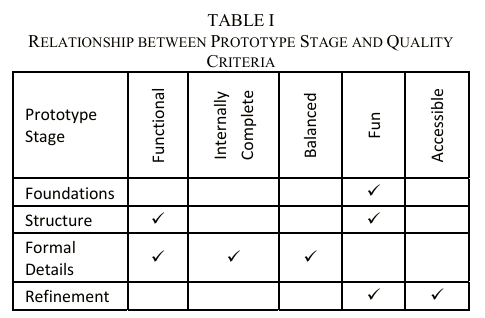
\includegraphics[scale=0.8]{image11.png}
  \caption{Relación entre etapas de prototipo y criterios de calidad. Extraída de \cite{ramadanGameDevelopmentLife2013}.}
  \label{fig:x relacion entre prototipo y criterios de calidad}
\end{figure}
\par Ramadan y Widyani \cite{ramadanGameDevelopmentLife2013} proponen conectar estos conceptos con las etapas del desarrollo de un videojuego. Las fases están siguen un modelo evolutivo, y están compuestas por:
\begin{enumerate}
    \item Initiation: en esta etapa se define la idea general del juego. Se escribe el concepto básico que se formalizará en las siguientes etapas.
    \item Ciclo: en esta fase se crea un documento de diseño y una serie de prototipos, siguiendo los parámetros establecidos por Fullerton \cite{fullertonGameDesignWorkshop2008}.
    \begin{enumerate}
        \item Pre-production: El primer prototipo es “Foundations”, que está relacionado con el criterio de “fun”. A partir de ahí, el resto de prototipos son llamados “Structure”, es decir que cumplen con los criterios de “fun” y “functional” \cite{ramadanGameDevelopmentLife2013}.
        \item Production: en esta etapa se crean los assets y se escribe el código del juego. De este proceso aparecen 2 prototipos 
        \begin{itemize}
            \item “Formal Details”: integra el arte y las mecánicas. Se obtiene un prototipo balanceado, con nuevas features y libre de bugs.
            \item “Refinement”: prototipo completo que busca cumplir con los criterios de “fun” y “accessible”.
        \end{itemize}
        \item Testing: en esta etapa se prueban los prototipos en la etapa anterior. El resultado de esta etapa indica si se pasa a la siguiente fase o si se vuelve a “pre-production”. Ramadan y Widyani \cite{ramadanGameDevelopmentLife2013} nombran 2 métodos de testing:
        \begin{itemize}
            \item Testing de “Formal Details”: se validan la funcionalidad de las mecánicas y la dificultad del juego (cumple con con el criterio “balanced”). Para ello, se realizan sesiones donde los testers juegan el juego y documentan los bugs que encuentren. Además se les pide que documenten cómo se sienten respecto a la dificultad del videojuego.
            \item Testing de “Refinement”: se valida que el prototipo cumple con los criterios de “fun” y “accessibility”. Esto también se realiza con sesiones de juego, pero en este caso se observa el comportamiento del jugador para notar si el prototipo es intuitivo o no.
        \end{itemize}
        \item Beta: en esta fase, se realizan pruebas utilizando testers externos a la empresa. Se utilizan los mismos métodos de la etapa anterior, y también puede resultar en volver a comenzar el ciclo de pre-producción. En caso de encontrar buena recepción, se continúa a la siguiente fase.
    \end{enumerate}
    \item Release: en esta etapa, el proyecto ya está listo para ser lanzado al público.
\end{enumerate}
\begin{figure}[H]
  \centering
  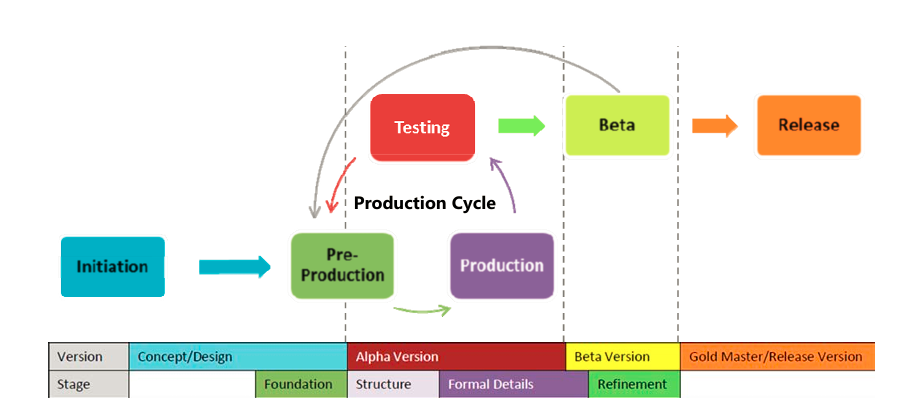
\includegraphics[scale=0.45]{image9.png}
  \caption{El ciclo de desarrollo propuesto por Ramadan y Widyani. Extraída de \cite{ramadanGameDevelopmentLife2013}.}
  \label{fig:x gdlc Ramadan y Widyani}
\end{figure}